% Created 2024-11-22 Fri 11:23
% Intended LaTeX compiler: pdflatex
\documentclass[aspectratio=169,xcolor={dvipsnames,svgnames}]{beamer}
\usepackage[utf8x]{inputenc}
\usepackage[T1]{fontenc}
\usepackage{graphicx}
\usepackage{longtable}
\usepackage{wrapfig}
\usepackage{rotating}
\usepackage[normalem]{ulem}
\usepackage{amsmath}
\usepackage{amssymb}
\usepackage{capt-of}
\usepackage{hyperref}
\usepackage{minted}
\usepackage{libertine}
\usepackage[normalem]{ulem}
\usepackage{varwidth}
\usepackage[Export]{adjustbox}
%\usepackage{enumitem}
\usepackage[linesnumbered,ruled,vlined]{algorithm2e}
\usepackage{tabularx}
\graphicspath{ {./images/} {./org-download-images/} }
\usepackage[date=year,%
backend=biber,%
style=alphabetic,%
maxnames=5,%
minnames=3,%
maxalphanames=4,%
minalphanames=3,%
backref=true,%
doi=false,%
isbn=false,%
url=false,%
eprint=false]{biblatex}
\DefineBibliographyStrings{english}{%
backrefpage  = {\lowercase{s}ee p.}, % for single page number
backrefpages = {\lowercase{s}ee pp.} % for multiple page numbers
}
\addbibresource{/home/bvraghav/bibliography.bib}
%% Math typesetting
%% --------------------------------
\usepackage{amsmath}
\usepackage{amssymb}
\usepackage{amsfonts}
\usepackage{bbold}
% Operators with limit-style sub and superscript
\DeclareMathOperator*{\E}{\mathbb{E}}
\hypersetup{%
colorlinks=true,%
allcolors=magenta,%
%linkbordercolor = {white},%
%<your other options...>,
}
\usetheme{boxes}
\usecolortheme{crane}
\usefonttheme{serif}
\useinnertheme{rectangles}
\useoutertheme{}
\date{\textit{[2024-08-19 Mon]}}
\title{jasper}
\subtitle{ucs749: speech processing and synthesis}
\author{%
%\noindent{} \\[2em]
\normalsize Raghav B. Venkataramaiyer
}
\institute{%
CSED TIET Patiala India.
}
\date{\scriptsize \today}
\setbeamercolor{alerted text}{fg=red!80!black}
%% Setup outline at begin section
%% -------------------------------------------------------
\AtBeginSection[]               % Section
{
\begin{frame}{outline}
\tableofcontents[currentsection,hideallsubsections]
\end{frame}
}
\AtBeginSubsection[]            % SubSection
{
\begin{frame}{outline}
\tableofcontents[currentsection,currentsubsection,subsectionstyle=show/shaded/hide]
\end{frame}
}
\setbeamerfont{structure}{shape=\scshape,family=\sffamily}
\setbeamertemplate{section page}
{
\begin{centering}
\begin{beamercolorbox}[sep=12pt,center]{part title}
\usebeamerfont{section title}\insertsection\par
\end{beamercolorbox}
\end{centering}
}

\setbeamercovered{transparent}
\hypersetup{
 pdfauthor={Raghav B. Venkataramaiyer},
 pdftitle={jasper},
 pdfkeywords={},
 pdfsubject={},
 pdfcreator={Emacs 29.4 (Org mode 9.6.24)}, 
 pdflang={English}}
\begin{document}

\maketitle

\section{metadata}
\label{sec:org38583d8}

\begin{frame}[label={sec:orgc325e05}]{metadata}
\begin{description}
\item[{tags}] Interspeech 2019
\item[{keywords}] Computer Science - Computation and
Language, Computer Science - Machine Learning,
Computer Science - Sound, Electrical Engineering and
Systems Science - Audio and Speech Processing
\item[{author}] Li, J., Lavrukhin, V., Ginsburg, B., Leary,
R., Kuchaiev, O., Cohen, J. M., Nguyen, H., […]
\item[{url}] \href{http://arxiv.org/abs/1904.03288}{[arXiv]​}, \href{https://paperswithcode.com/paper/jasper-an-end-to-end-convolutional-neural\#code}{[Papers With Code]​}
\end{description}
\end{frame}

\section{prior art}
\label{sec:prior-art}
\begin{frame}[label={sec:datasets}]{datasets}
\begin{itemize}
\item \href{https://doi.org/10.1109/ICASSP.2015.7178964}{LibriSpeech (ICASSP ’15)}
\item WSJ: \href{https://doi.org/10.35111/ewkm-cg47}{LDC93S6A (WSJ0)}, \href{https://doi.org/10.35111/q7sb-vv12}{LDC94S13A (WSJ1)}
\item 2000hr Fisher+Switchboard (F+S): \href{https://doi.org/10.35111/da4a-se30}{LDC2004S13},
\href{https://doi.org/10.35111/dz78-gx84}{LDC2005S13}, \href{https://doi.org/10.35111/sw3h-rw02}{LDC97S62}
\end{itemize}
\end{frame}


\begin{frame}[label={sec:ideas-and-strategy}]{ideas and strategy}
\begin{itemize}
\item \href{../time-delay-networks/}{Time-delay Networks (TDNN)} \href{https://www.cs.toronto.edu/\~hinton/absps/langTDNN.pdf}{[PDF}]
\item \href{../ctc/}{Connectionist Temporal Classification (CTC) ICML ’06}
\href{https://dl.acm.org/doi/abs/10.1145/1143844.1143891}{[ACM}]
\item \href{https://arxiv.org/abs/1609.03193}{Wav2Letter (ICLR '17)}
\item \hyperlink{sec:gated-activation-unit}{Gated Convnets (for ASR)} \href{https://arxiv.org/abs/1712.09444}{[arXiv}]
\end{itemize}
\end{frame}

\begin{frame}[label={sec:technology}]{technology}
\begin{description}
\item[{Normalisation}] \begin{itemize}
\item \hyperlink{sec:batch-norm}{Batch Norm}; See also:\href{https://arxiv.org/abs/1502.03167}{[arXiv];}
\item \hyperlink{sec:weight-norm}{Weight Norm}; See also: \href{http://arxiv.org/abs/1602.07868}{[arXiv];}
\item \hyperlink{sec:layer-norm}{Layer Norm}; See also: \href{http://arxiv.org/abs/1607.06450}{[arXiv];}
\end{itemize}
\item[{Activation}] \begin{itemize}
\item \hyperlink{sec:orgf33426f}{ReLU}
\item \hyperlink{sec:orgf33426f}{Clipped ReLU}
\item \hyperlink{sec:orgf33426f}{Leaky ReLU}
\end{itemize}
\item[{Gated Units}] \begin{itemize}
\item \hyperlink{sec:gated-linear-unit}{Gated Linear Units}
\item \hyperlink{sec:gated-activation-unit}{Gated Activation Units}
\end{itemize}
\end{description}
\end{frame}

\section{Contribution}
\label{sec:org7d6064a}
\begin{frame}[label={sec:contribution}]{Contribution}
\begin{itemize}
\item Jasper Model; and Dense Residual Topology;
\item Evidence-based insights on convergence and
non-convergence;
\item NovoGrad Solver (like Adam);
\item WER improvement on LibriSpeech test-clean.
\end{itemize}
\end{frame}

\begin{frame}[label={sec:jasper-model}]{jasper model}
All figures and tables repeated here from the paper
[LLGL+19].

Model search across
\begin{description}
\item[{3 types of normalisation}] \hyperlink{sec:batch-norm}{Batch Norm}, \hyperlink{sec:weight-norm}{Weight Norm},
\hyperlink{sec:layer-norm}{Layer Norm};
\item[{3 types of activations}] \hyperlink{sec:orgf33426f}{ReLU, clipped ReLU, Leaky
ReLU};
\item[{2 types of Gates}] \hyperlink{sec:gated-linear-unit}{Gated Linear Units}, \hyperlink{sec:gated-activation-unit}{Gated
Activation Units};
\item[{Architecture}] \hyperlink{sec:jasper-b-times-r-architecture}{\(B\times R\) parameterisation}, \hyperlink{sec:jasper-dense-residual-architecture}{Dense
Residual}.
\end{description}
\end{frame}



\begin{frame}[label={sec:jasper-b-times-r-architecture}]{jasper \(B\times R\) architecture}
\begin{columns}
\begin{column}{0.4\columnwidth}
\begin{figure}[htbp]
\centering
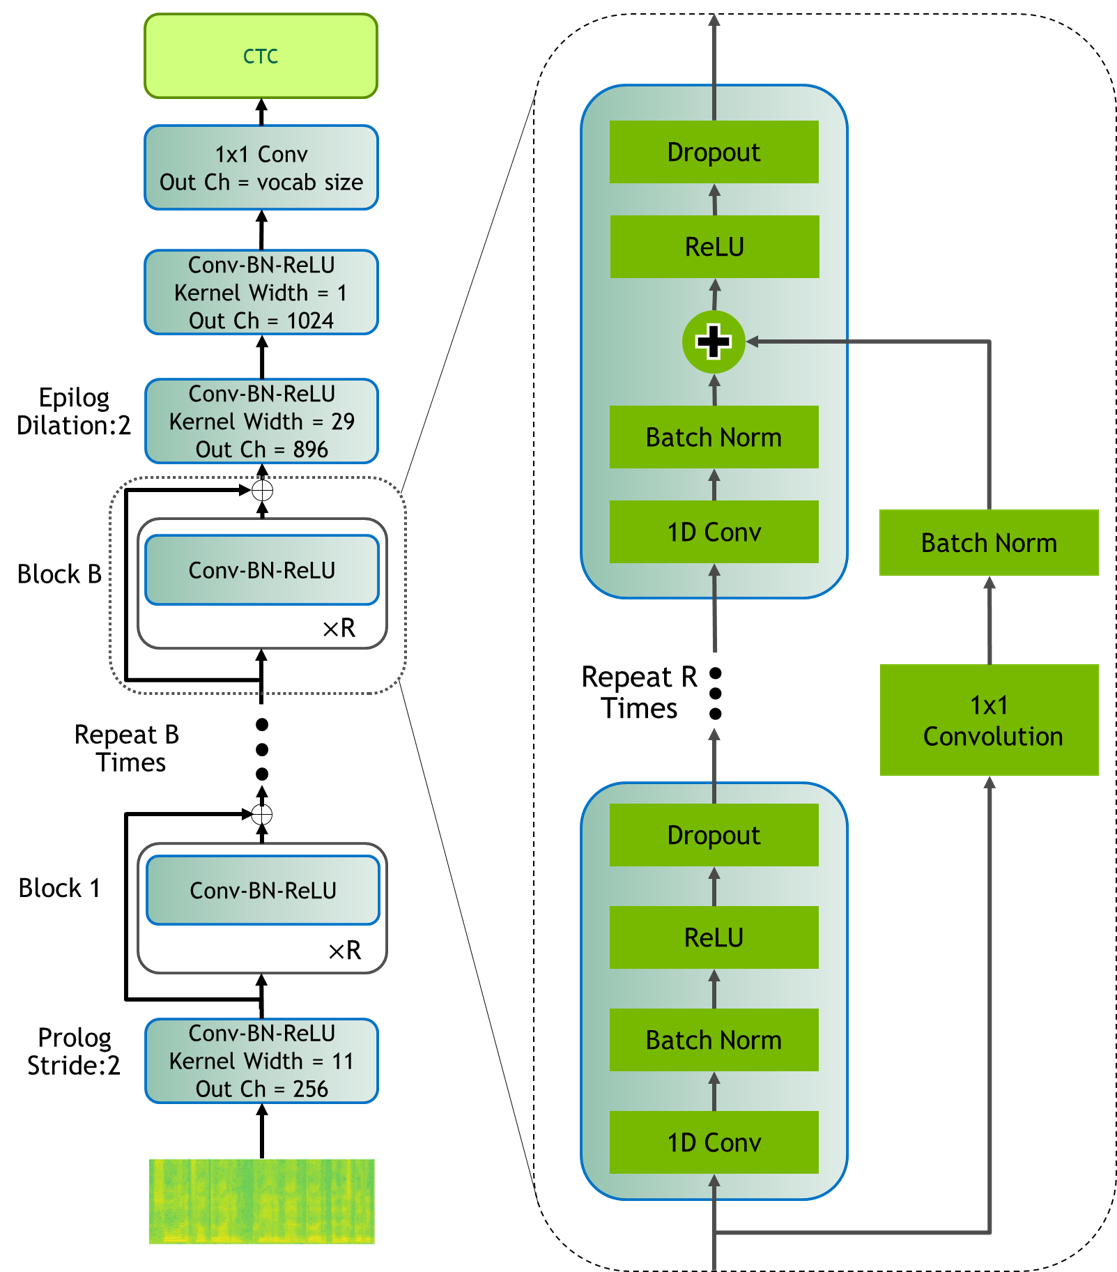
\includegraphics[width=.9\linewidth]{org-download-images/Contribution/2024-08-28_07-44-17_screenshot.png}
\caption{Jasper \(B\times R\) model: \(B\): number of blocks; \(R\): number of sub-blocks.}
\end{figure}
\end{column}

\begin{column}{0.6\columnwidth}
\begin{table}[htbp]
\caption{Jasper \(10\times 5\)}
\centering
\begin{tabular}{rrlrrr}
\hline
\#B & \#S & B & K & \#C (out) & Dropout\\[0pt]
\hline
1 & 1 & Conv1 & 11 (s=2) & 256 & 0.2\\[0pt]
\hline
2 & 5 & B1 & 11 & 256 & 0.2\\[0pt]
2 & 5 & B2 & 13 & 384 & 0.2\\[0pt]
2 & 5 & B3 & 17 & 512 & 0.2\\[0pt]
2 & 5 & B4 & 21 & 640 & 0.3\\[0pt]
2 & 5 & B5 & 25 & 768 & 0.3\\[0pt]
\hline
1 & 1 & Conv2 & 29 (D=2) & 896 & 0.4\\[0pt]
1 & 1 & Conv3 & 1 & 1024 & 0.4\\[0pt]
1 & 1 & Conv4 & 1 & \#graphemes & 0\\[0pt]
\hline
\end{tabular}
\end{table}
\end{column}
\end{columns}
\end{frame}


\begin{frame}[label={sec:org6c6d0bc}]{fundamental conv block}
\begin{columns}
\begin{column}{0.2\columnwidth}
\begin{center}
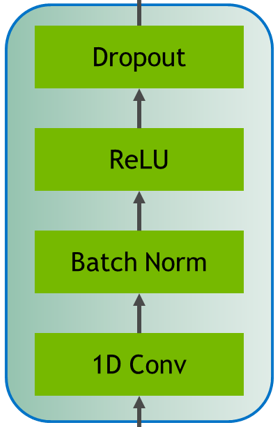
\includegraphics[width=.9\linewidth]{org-download-images/Contribution/2024-09-16_22-58-22_screenshot.png}
\end{center}
\end{column}

\begin{column}{0.8\columnwidth}
The fundamental conv block with \\[0pt]
Conv \(\mapsto\) Batch Norm \(\mapsto\) ReLU \(\mapsto\)
Dropout \\[0pt]
progression
\end{column}
\end{columns}
\end{frame}

\begin{frame}[label={sec:orga5b98e6}]{jasper block}
\begin{columns}
\begin{column}{0.25\columnwidth}
\begin{center}
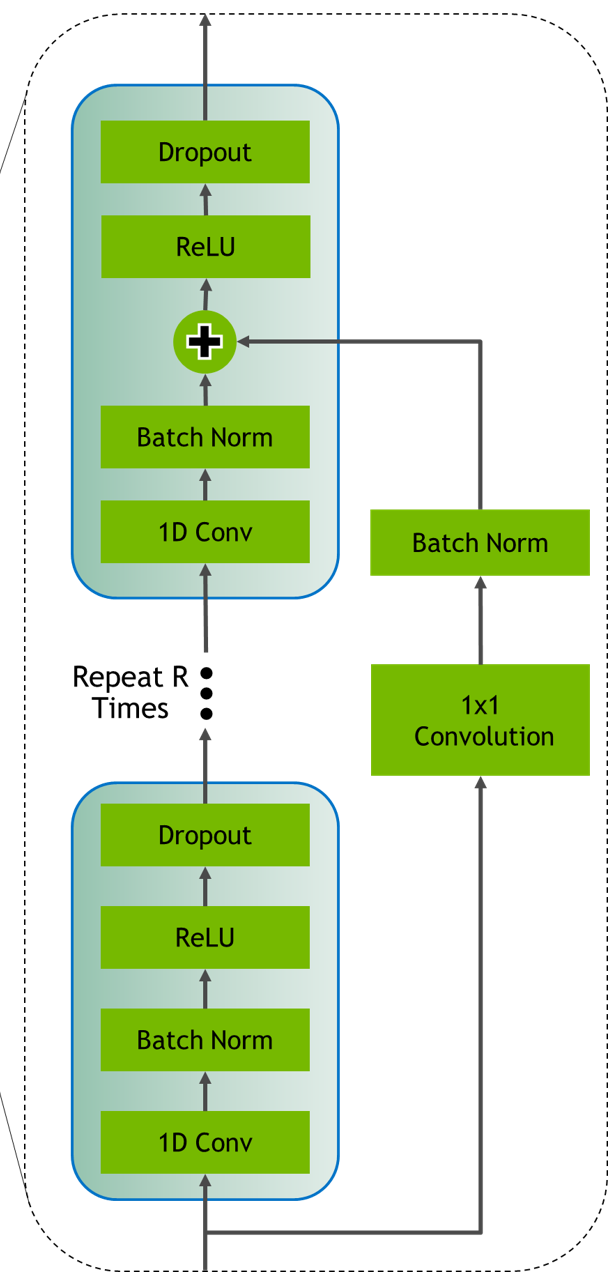
\includegraphics[width=.9\linewidth]{org-download-images/Contribution/2024-09-16_23-01-42_screenshot.png}
\end{center}
\end{column}
\begin{column}{0.6\columnwidth}
The fundamental Conv Block (aka Sub-Block) is repeated
\(R\) times, with a residual connection from inputs to
the final block as in figure, to create a Jasper Block.
\end{column}
\end{columns}
\end{frame}

\begin{frame}[label={sec:orge99d87b}]{\(B\times R\) again}
\begin{columns}
\begin{column}{0.45\columnwidth}
\begin{center}
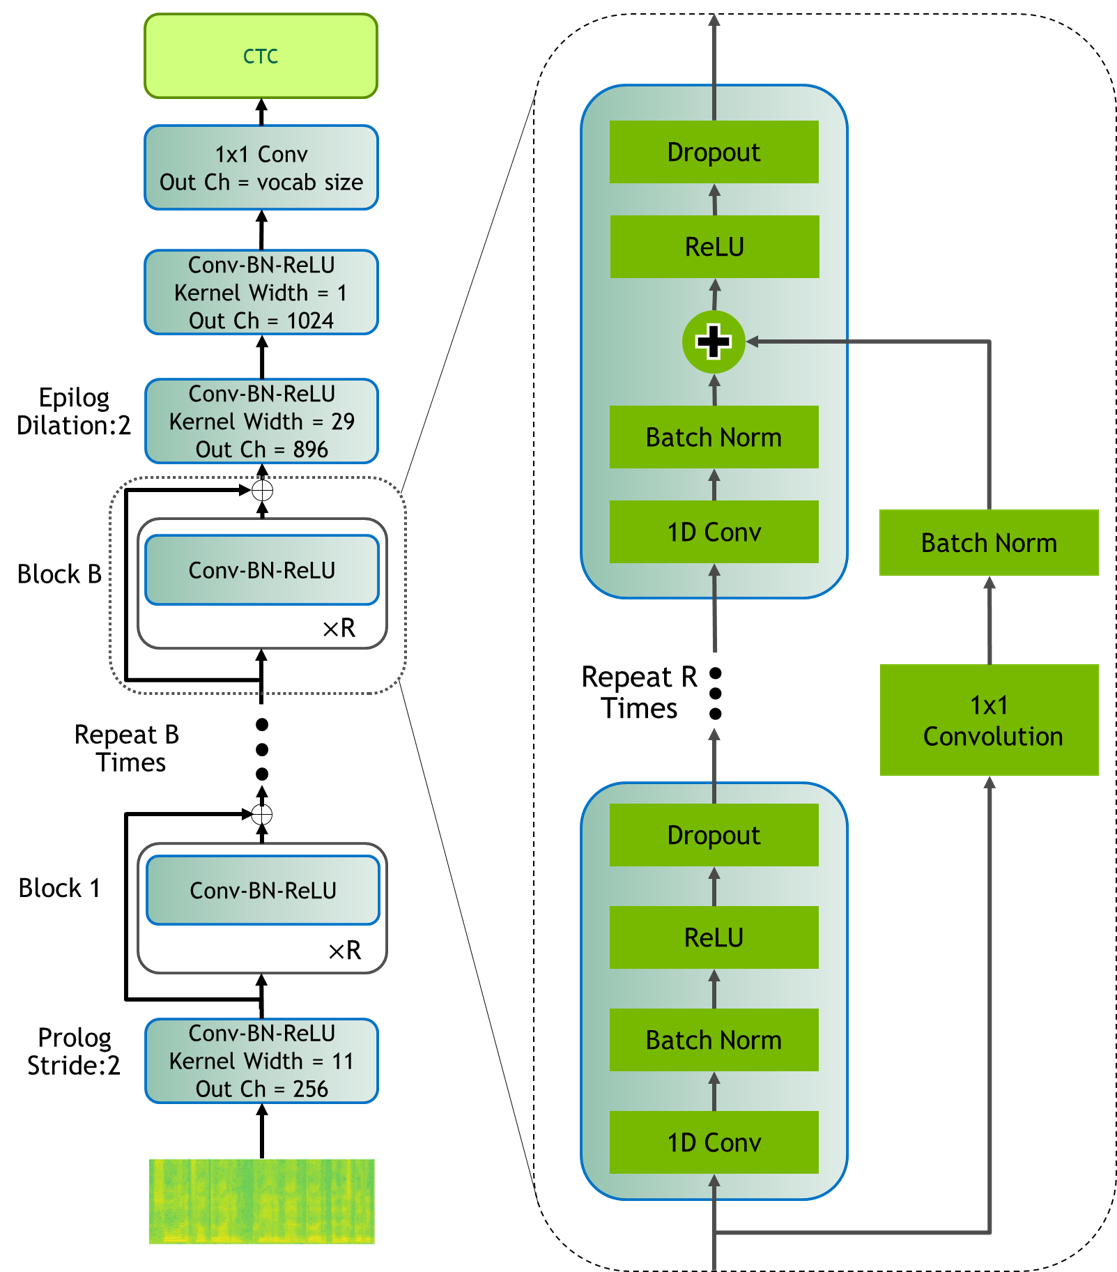
\includegraphics[width=.9\linewidth]{org-download-images/Contribution/2024-08-28_07-44-17_screenshot.png}
\end{center}
\end{column}

\begin{column}{0.55\columnwidth}
The Jasper Block is repeated \(B\) times to create the
\(B\times R\) architecture.
\end{column}
\end{columns}
\end{frame}

\begin{frame}[label={sec:jasper-dense-residual-architecture}]{jasper dense residual architecture}
\begin{columns}
\begin{column}{0.45\columnwidth}
\begin{figure}[htbp]
\centering
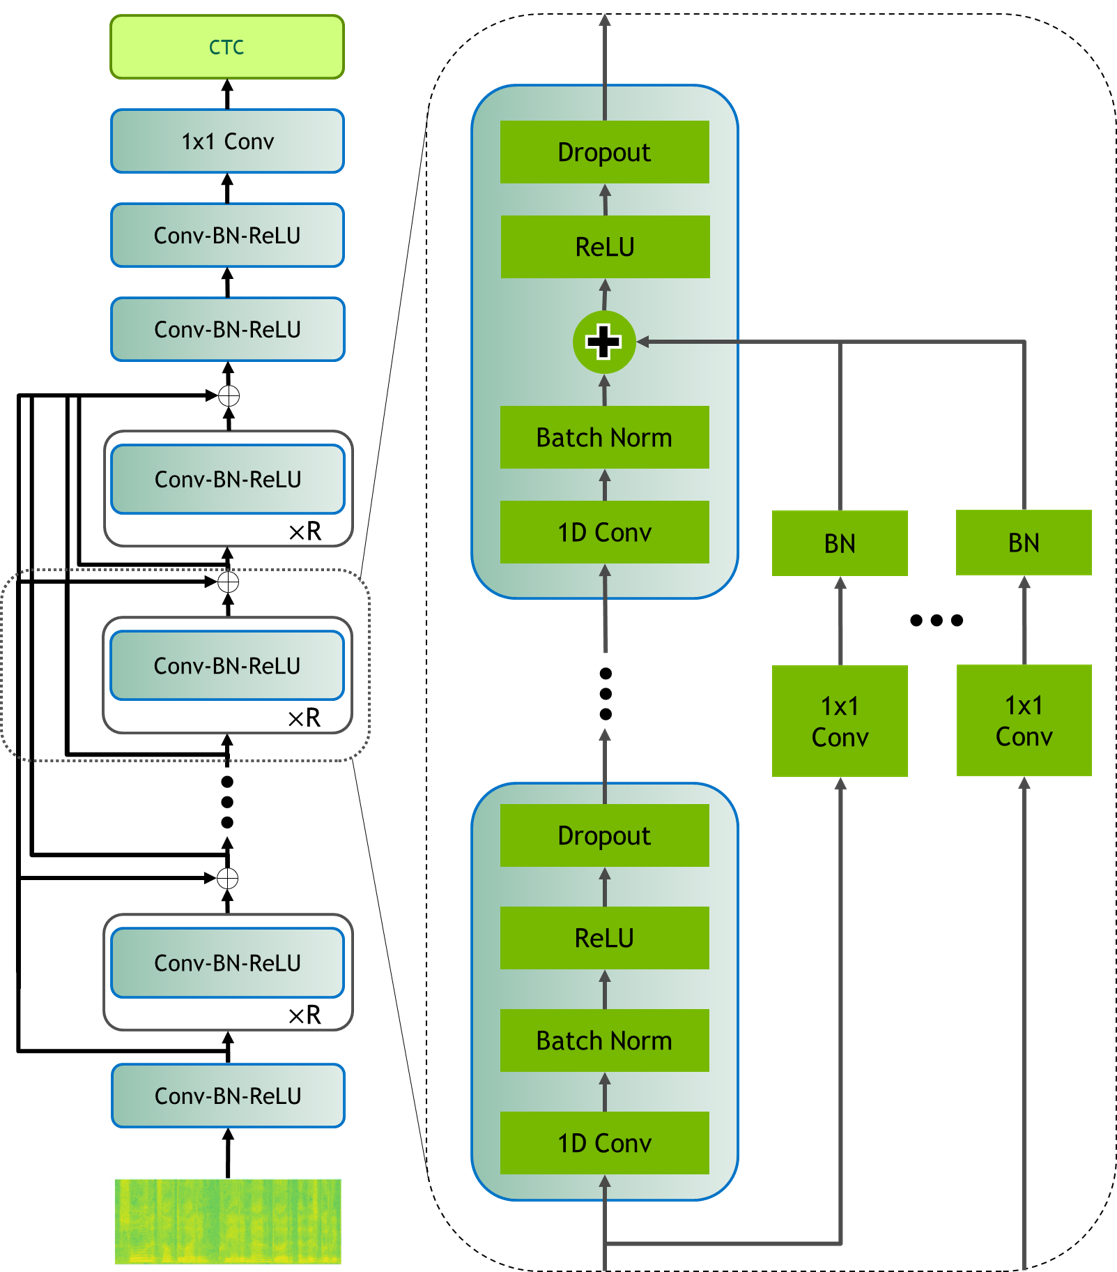
\includegraphics[width=.9\linewidth]{org-download-images/Contribution/2024-08-28_07-46-36_screenshot.png}
\caption{Jasper Dense Residual Model}
\end{figure}
\end{column}

\begin{column}{0.55\columnwidth}
\begin{itemize}
\item The dense residual architecture builds on top of
jasper residual architecture; and
\item provides skip connections to the final block from
each of the previous blocks.
\item \emph{I.e.} within a block, the final sub-block receives a
skip-connection from each of the previous sub-blocks; and
\item on the whole, the final block receives skip
connections from each of the previous blocks.
\end{itemize}
\end{column}
\end{columns}
\end{frame}


\section{details}
\label{sec:appendix}
\subsection{Normalisation}
\label{sec:org70d8189}

\begin{frame}[label={sec:covariate-shift}]{covariate shift}
\begin{columns}
\begin{column}{0.45\columnwidth}
\begin{quote}
One of the challenges of deep learning is that the
gradients with respect to the weights in one layer are
highly dependent on the outputs of the neurons in the
previous layer especially if these outputs change in a
highly correlated way. \\[0pt]
--- \href{http://arxiv.org/abs/1607.06450}{Layer Normalisation Paper}
\end{quote}
\end{column}
\end{columns}
\end{frame}

\begin{frame}[label={sec:batch-norm}]{batch norm}
\begin{columns}
\begin{column}{0.5\columnwidth}
\begin{figure}[htbp]
\centering
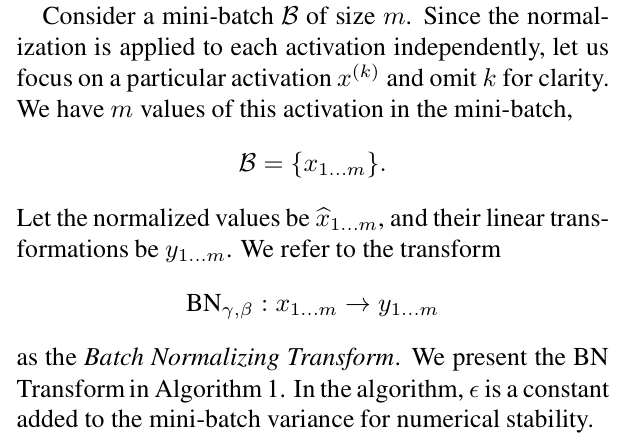
\includegraphics[width=.9\linewidth]{org-download-images/details/2024-09-16_23-14-37_screenshot.png}
\caption{\label{fig:batch-norm}Courtesy: \href{https://arxiv.org/abs/1502.03167}{Batch Norm Paper}}
\end{figure}
\end{column}

\begin{column}{0.5\columnwidth}
\begin{center}
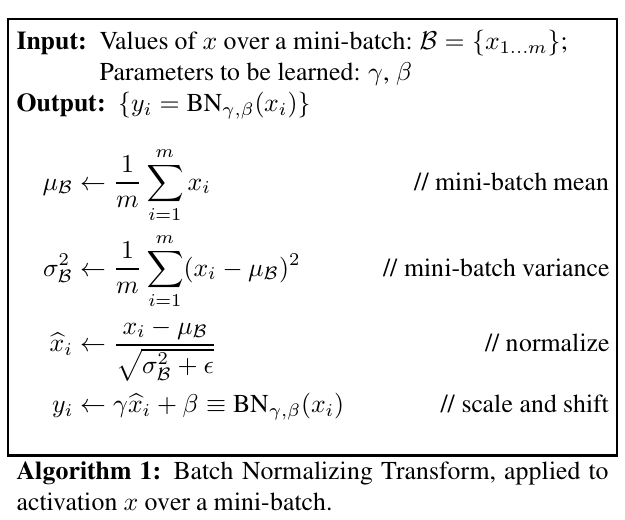
\includegraphics[width=.9\linewidth]{org-download-images/details/2024-09-16_23-15-12_screenshot.png}
\end{center}
\end{column}
\end{columns}
\end{frame}

\begin{frame}[label={sec:weight-norm}]{weight norm}
\begin{columns}
\begin{column}{0.7\columnwidth}
Each neuron on an artificial neural network may be
represented as,

\begin{align}
\notag
y &= \phi(\mathbf{w}\cdot\mathbf{x}+b)
\end{align}

where, \\[0pt]
\(\mathbf{x}\) is \(k\) dimensional vector of input
features, \\[0pt]
\(\mathbf{w}\) is \(k\) dimensional vector of learnable
weights, \\[0pt]
\(b\) is a (learnable) scalar bias term, and \\[0pt]
\(\phi\) denotes element-wise non-linearity.
\end{column}
\end{columns}
\end{frame}

\begin{frame}[label={sec:org30dd335}]{weight norm}
\begin{columns}
\begin{column}{0.45\columnwidth}
The \alert{key idea} in weight normalisation is to
re-parameterise the weight vector, as
\begin{align}
  \notag
  \mathbf{w} &= \frac{g}{\|\mathbf{v}\|} \mathbf{v}
\end{align}
so that, \\[0pt]
\(\mathbf{v}\) is \(k\) dimensional vector of learnable
weights, \\[0pt]
\(g\) is a learnable scalar parameter, and 
\(\|\mathbf{w}\|=g\), independent of \(\mathbf{v}\).
\end{column}
\end{columns}
\end{frame}
\begin{frame}[label={sec:org8c73af7}]{weight norm}
\begin{columns}
\begin{column}{0.45\columnwidth}
Instead of working with \(g\) directly, we may also use
an exponential parameterisation for the scale,
\begin{align}
  \notag
  g &= e^s
\end{align}
where, \(s\) is a log-scale learnable scalar parameter.

For more details, please see \(\S 2.1\) and \(\S 2.2\) of
the \href{http://arxiv.org/abs/1602.07868}{weight norm paper}.
\end{column}
\end{columns}
\end{frame}

\begin{frame}[label={sec:layer-norm}]{layer norm}
Summarising Batch Norm
\begin{columns}
\begin{column}{0.7\columnwidth}
The \(l^{\text{th}}\) layer in a feed forward neural
network with inputs \(\mathbf{h}^l\) and weight matrix
\(W^{l}\) and non-linear activation \(f\), may be written
as,
\begin{align}
  \notag
  a_i^l &= {\mathbf{w}_{:,i}^l}^\top\mathbf{h}^l
          \qquad h_i^{l+1} = f(a_i^l+b_i^l) 
\end{align}

A Batch Norm may be summarised as,
\begin{align}
  \notag
  h_i^{l+1} = f(\hat{a}_i^l+b_i^l)
  &\qquad
    \hat{a}_i^l = \frac{g_i^l}{\sigma_i^l} (a_i^l -
    \mu_i^l) \\
  \notag
  \mu_i^l = \underset{\mathbf{x}\sim P(\mathbf{x})}
  {\mathbb{E}} \left[a_i^l\right]
  &\qquad
    \sigma_i^l = \sqrt{\underset{\mathbf{x}\sim
    P(\mathbf{x})} {\mathbb{E}} \left[\left(a_i^l -
    \mu_i^l\right)^2\right]}
\end{align}
\end{column}
\end{columns}
\end{frame}

\begin{frame}[label={sec:org38547fc}]{layer norm}
\begin{columns}
\begin{column}{0.45\columnwidth}
A Batch Norm may be summarised as,
\begin{align}
  \notag
  h_i^{l+1} &= f(\hat{a}_i^l+b_i^l) \\
  \notag
  \hat{a}_i^l &= \frac{g_i^l}{\sigma_i^l} (a_i^l -
  \mu_i^l) \\
  \notag
  \mu_i^l &= \underset{\mathbf{x}\sim P(\mathbf{x})}
  {\mathbb{E}} \left[a_i^l\right] \\
  \notag
  \sigma_i^l &= \sqrt{\underset{\mathbf{x}\sim
  P(\mathbf{x})} {\mathbb{E}} \left[\left(a_i^l -
  \mu_i^l\right)^2\right]}
\end{align}
\end{column}


\begin{column}{0.55\columnwidth}
The authors say,
\begin{itemize}
\item It is typically impractical to [exactly] compute the
expectations [in the adjoining eqn's]; since
\item it would require forward passes through the whole
training dataset with the current set of weights;
\item Instead, \(\mu\) and \(\sigma\) are estimated using the
empirical samples from the current mini-batch.
\end{itemize}
\end{column}
\end{columns}
\end{frame}

\begin{frame}[label={sec:org99a409e}]{layer norm}
\begin{columns}
\begin{column}{0.45\columnwidth}
In certain cases, the covariate shift is was observed
to be more profound at layer level by the authors.  The
authors say,

\begin{quote}
[\ldots] Notice that changes in the output of one layer
will tend to cause highly correlated changes in the
summed inputs to the next layer, especially with ReLU
units whose outputs can change by a lot.
\end{quote}
\end{column}
\begin{column}{0.55\columnwidth}
\begin{quote}
We, thus, compute the layer normalization statistics
over \alert{all the hidden units} in the same layer as
follows:
\end{quote}

\begin{align}
  \notag
  \mu_i^l = \mu^l
  &= \frac1H\sum_{i=1}^{H}a_i^l \\
  \notag
  \sigma_i^l = \sigma^l
  &= \sqrt{ \frac1H \sum_{i=1}^H \left( a_i^l - \mu^l
    \right)^{2}}
\end{align}

\emph{i.e.} \(\mu^{l}\) and \(\sigma^{l}\) are same for all
neurons in the same layer.
\end{column}
\end{columns}
\end{frame}

\begin{frame}[label={sec:org2d30b25}]{comparing normalisation mechanisms}
\begin{figure}[htbp]
\centering
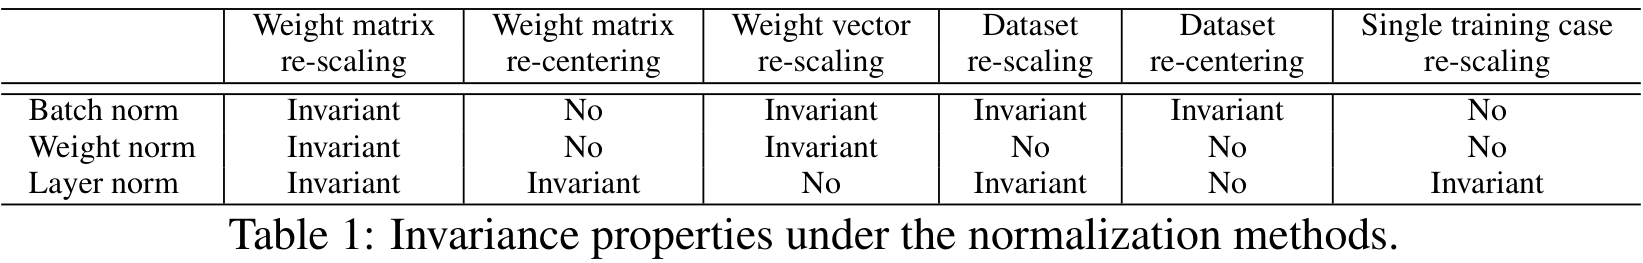
\includegraphics[width=.9\linewidth]{org-download-images/Appendix/2024-08-20_03-20-24_screenshot.png}
\caption{Courtesy: \href{http://arxiv.org/abs/1607.06450}{Layer Norm Paper}}
\end{figure}
\end{frame}

\subsection{Sigmoid Activation}
\label{sec:sigmoid-activation}
\begin{frame}[label={sec:error-function}]{error function}
\begin{columns}
\begin{column}{0.65\columnwidth}
\begin{figure}[htbp]
\centering
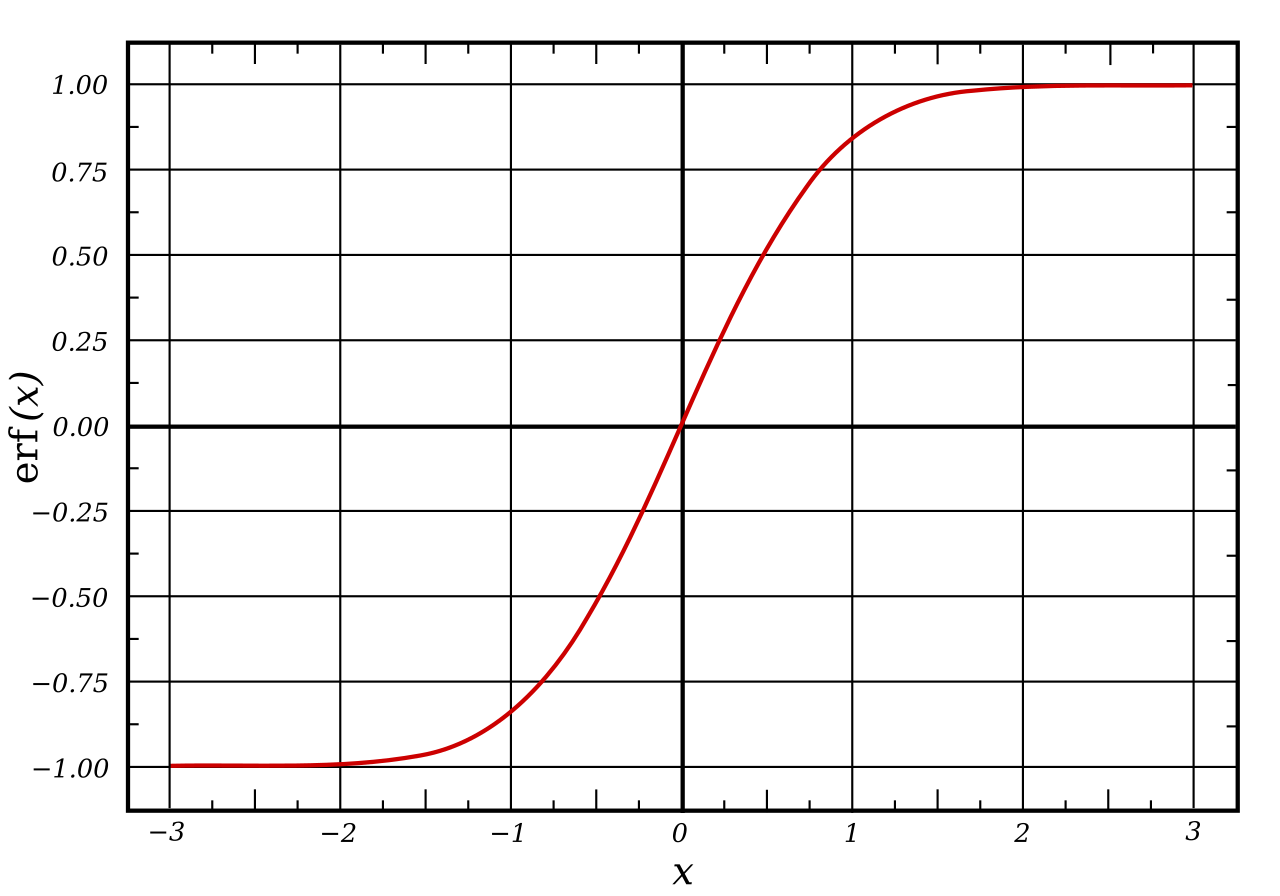
\includegraphics[width=.9\linewidth]{org-download-images/details/2024-09-16_22-48-51_screenshot.png}
\caption{Image Courtesy: \href{https://commons.wikimedia.org/wiki/File:Error\_Function.svg}{Wikipedia}}
\end{figure}
\end{column}

\begin{column}{0.35\columnwidth}
\begin{align}
  \notag
  \mathrm{erf}\;z &= \frac2{\sqrt\pi} \int_0^z e^{-t^2}
                   \mathrm{d}t 
\end{align}
\end{column}
\end{columns}
\end{frame}


\begin{frame}[label={sec:sigmoid-logistic-function}]{sigmoid (logistic Function)}
\begin{columns}
\begin{column}{0.65\columnwidth}
\begin{figure}[htbp]
\centering
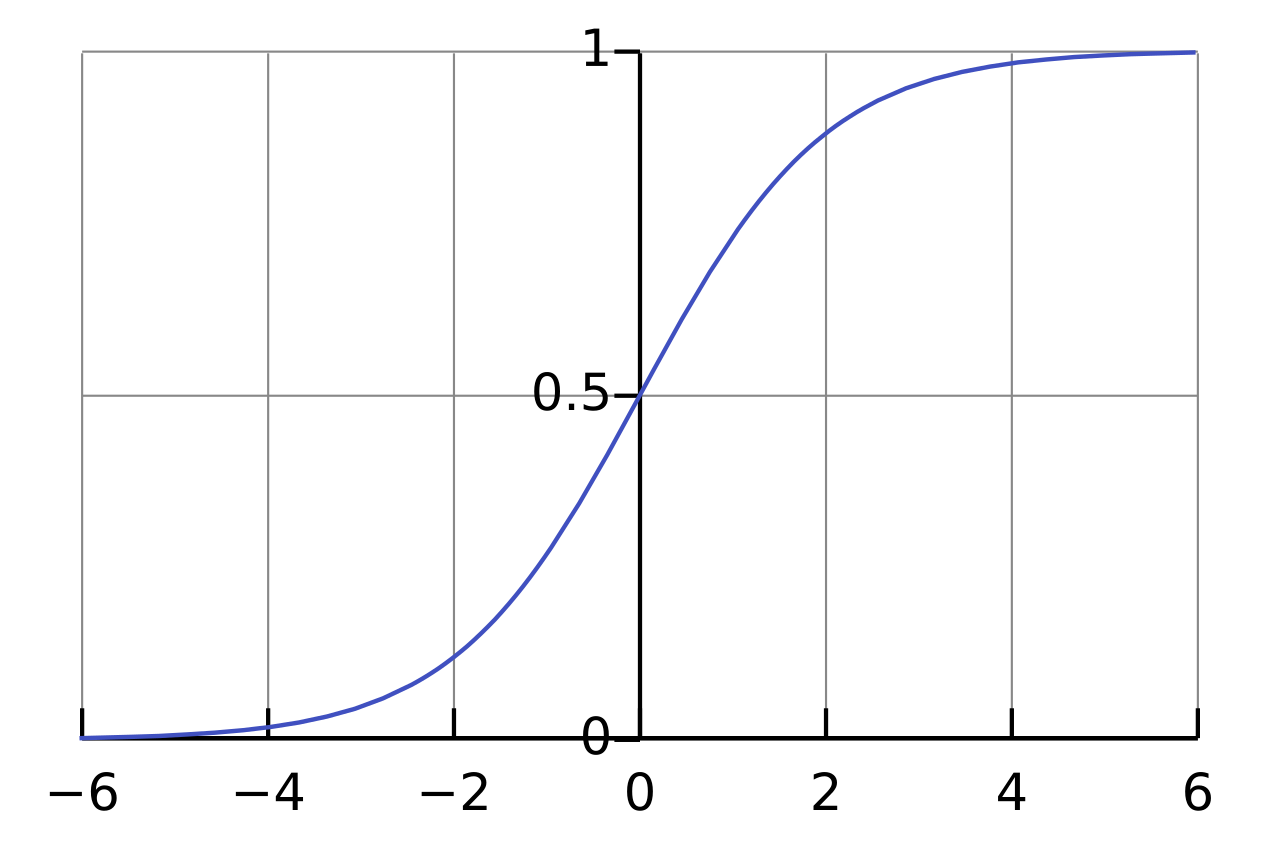
\includegraphics[width=.9\linewidth]{org-download-images/details/2024-09-16_22-50-24_screenshot.png}
\caption{Image Courtesy: \href{https://commons.wikimedia.org/wiki/File:Logistic-curve.svg}{Wikipedia}}
\end{figure}
\end{column}

\begin{column}{0.35\columnwidth}
\begin{align}
  \notag
  \sigma(x)
  &= \frac1{1+e^{-x} } \\
  \notag
  &= \frac{e^x}{1+e^x} \\
  \notag
  &= 1 - \sigma(-x)
\end{align}
\end{column}
\end{columns}
\end{frame}



\begin{frame}[label={sec:other-sigmoidal-functions}]{other sigmoidal Functions}
\begin{columns}
\begin{column}{0.65\columnwidth}
\begin{figure}[htbp]
\centering
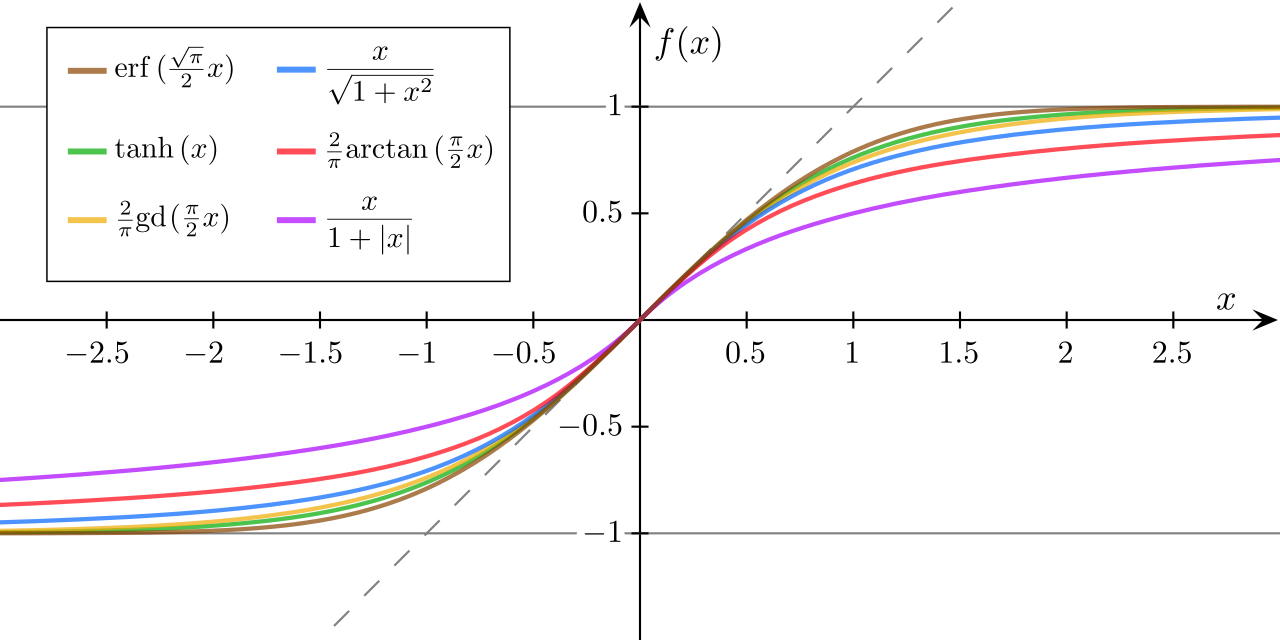
\includegraphics[width=.9\linewidth]{org-download-images/details/2024-09-16_22-51-13_screenshot.png}
\caption{Image Courtesy: \href{https://commons.wikimedia.org/wiki/File:Gjl-t(x).svg}{Wikipedia}}
\end{figure}
\end{column}

\begin{column}{0.35\columnwidth}
\begin{itemize}[<only@+>]
\item Hyperbolic Tangent
\begin{align}
  \notag
  \mathrm{tanh}\;x
  &= \frac {e^x - e^{-x}}{e^x + e^{-x}}
\end{align}
\item Arc Tangent
\begin{align*}
  y &= \mathrm{arctan}\;x \\
  \iff x &= \tan y; \\
  y &\in \left[-\frac\pi2,\frac\pi2\right]
\end{align*}
\item Gudermannian Function
\begin{align*}
  \notag
  \mathrm{gd}(x)
  &=\int_0^x \frac{\mathrm{d}t}{\mathrm{cosh}\;t} \\
  &= 2\;\mathrm{arctan}\left(\mathrm{tanh}\left(\frac
    x2 \right) \right)
\end{align*}
\item Algebraic Functions
\begin{align}
  \notag
  f(x) &= \frac{x}{\left(1+|x|^k\right)^{1/k}} \\
  \notag
  &= \frac{x}{\left(1+|x|\right)}; \qquad k=1 \\
  \notag
  &= \frac{x}{\sqrt{1+x^2}}; \qquad k=2
\end{align}
\end{itemize}
\end{column}
\end{columns}
\end{frame}


\subsection{Rectifier Activation}
\label{sec:orgf33426f}
\begin{frame}[label={sec:rectifier-activation}]{rectifier}
\begin{columns}
\begin{column}{0.45\columnwidth}
\begin{figure}[htbp]
\centering
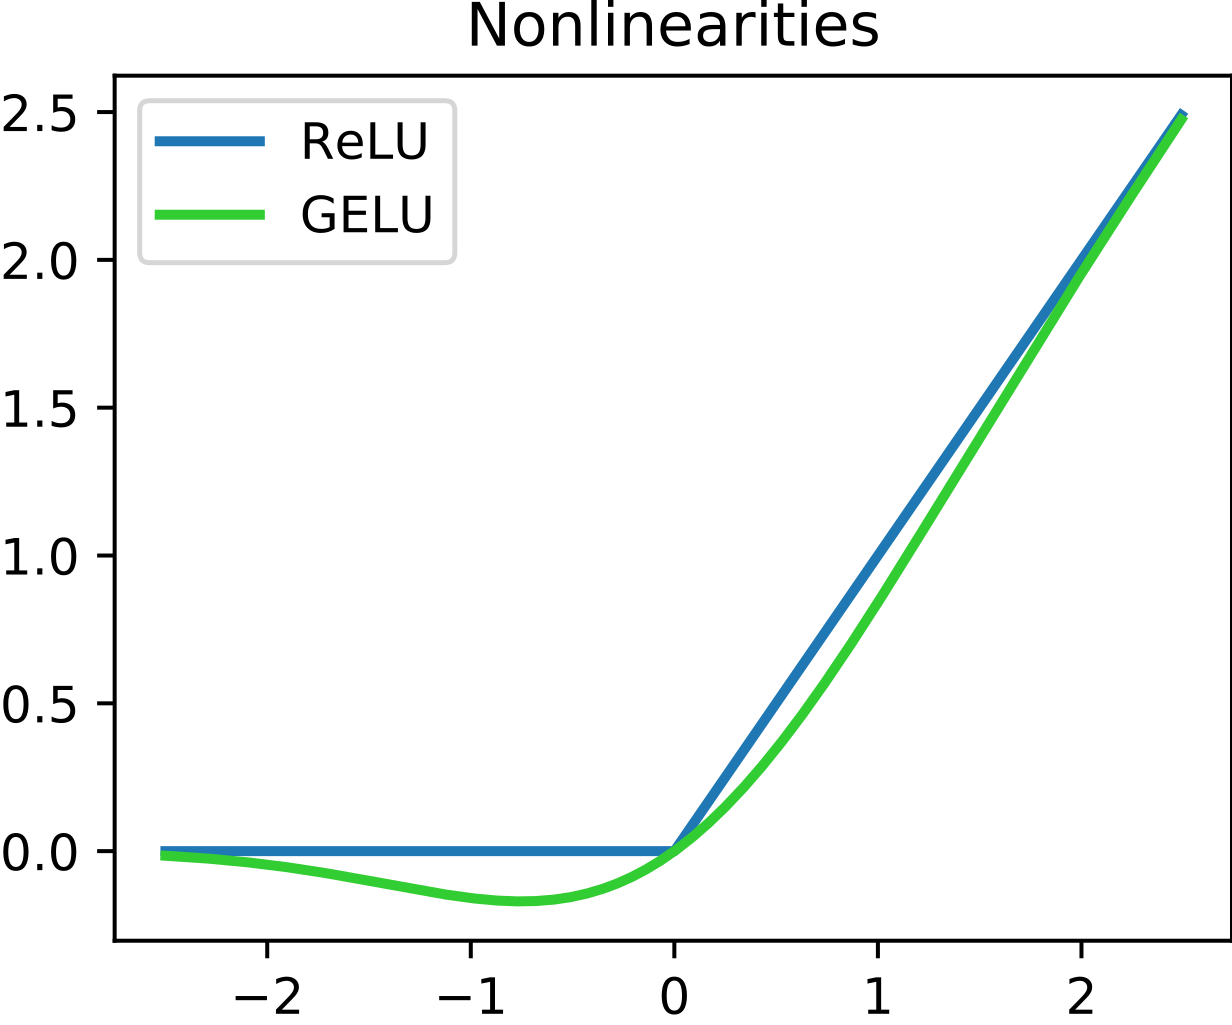
\includegraphics[width=.9\linewidth]{org-download-images/details/2024-09-16_22-52-05_screenshot.png}
\caption{Image Courtesy: \href{https://commons.wikimedia.org/wiki/File:ReLU\_and\_GELU.svg}{Wikipedia}}
\end{figure}
\end{column}

\begin{column}{0.55\columnwidth}
\begin{itemize}[<only@+>]
\item ReLU (Rectified Linear Unit)
\begin{align*}
  \notag
  \mathrm{ReLU}(x)
  &= x^+ \\
  &= \max(0,x) \\
  &= \frac{x+|x|}2 \\
  &= \begin{cases}
    x;&\text{if } x>0, \\
    0;&\text{otherwise.}
  \end{cases}
\end{align*}
\item Clipped ReLU
\begin{align}
  \notag
  \mathrm{cReLU}(x;a) &= \max(0,\min(a,x))
\end{align}
\emph{e.g.} ReLU6 in \href{https://pytorch.org/docs/stable/generated/torch.nn.ReLU6.html\#relu6}{[Pytorch]​}, \href{https://keras.io/api/layers/activations/\#relu6-function}{[Keras]​}
\item Parametric and Leaky ReLU
\begin{align}
  \notag
  \mathrm{PReLU}(x; a)
  &= \begin{cases}
    x;&\text{if } x>0, \\
    ax;&\text{otherwise.}
  \end{cases} \\
  \notag
  \mathrm{LeakyReLU}(x)
  &= \mathrm{PReLU}(x, 0.01)
\end{align}
\item GELU (Gaussian-error linear unit)
\begin{align}
  \notag
  GELU(x) &= x\cdot\Phi(x) \\
  \notag
  \frac\partial{\partial x} GELU(x)
  &= x\cdot\Phi'(x) + \Phi(x)
\end{align}
where \(\Phi(x) = Pr(X\leqslant x)\) is the cumulative
Gaussian distribution.
\end{itemize}
\end{column}
\end{columns}
\end{frame}

\subsection{Gating}
\label{sec:orgdd39034}
\begin{frame}[label={sec:vanishing-exploding-gradient-problem}]{vanishing/exploding gradient problem}
\begin{columns}
\begin{column}{0.7\columnwidth}
\begin{quote}
\href{https://doi.org/10.1109/9780470544037.ch14}{Hochreiter's work} formally identified a major reason:
Typical deep NNs suffer from the now famous problem of
vanishing or exploding gradients. With standard
activation functions (Sec. 1), cumulative
backpropagated error signals (Sec. 5.5.1) either shrink
rapidly, or grow out of bounds. In fact, they decay
\alert{exponentially} in the number of layers or CAP depth
(Sec. 3), or they explode. This is also known as the
long time lag problem.
\end{quote}
\alert{See also:} \href{https://arxiv.org/abs/1404.7828}{Deep Learning by Jurgen Schmidhuber}
\end{column}
\end{columns}
\end{frame}

\begin{frame}[label={sec:gating-history}]{gating history}
\begin{columns}
\begin{column}{0.7\columnwidth}
\begin{itemize}
\item Gating was introduced in the \href{https://ieeexplore.ieee.org/abstract/document/6795963}{LSTM paper} in '97, in
order to address vanishing/exploding gradient
problem.
\item Simply put, gating mechanism is element-wise
multiplication of input vector with a gate-activation
vector.
\end{itemize}
\end{column}
\end{columns}
\end{frame}
\begin{frame}[label={sec:org46e0046}]{gating history}
\begin{columns}
\begin{column}{0.7\columnwidth}
\begin{itemize}
\item The gate, in turn, is activated by looking at the
input vector itself.  For example, a basic gate would
be formulated as,
\end{itemize}

\begin{align}
  \notag
  \mathbf{y} &= \mathbf{g} \otimes \mathbf{x} \\
  \notag
  \mathbf{g} &= \sigma_{\otimes}(W\mathbf{x} +
               \mathbf{b}) 
\end{align}
where, \\[0pt]
\(\sigma_{\otimes}(\mathbf{x})\) is the element-wise
sigmoid activation of input vector \(\mathbf{x}\); and \\[0pt]
\(\otimes\) represents element-wise multiplication.
\end{column}
\end{columns}
\end{frame}

\begin{frame}[label={sec:org9d696b5}]{gating history}
\begin{columns}
\begin{column}{0.7\columnwidth}
For a more involved use-case, let an RNN be defined for
\(T\) time steps, with
\begin{itemize}
\item Given inputs as
\(\{\mathbf{z}_1,\ldots,\mathbf{z}_T\}\);
\item Cell States, \(\{\mathbf{c}_1,\ldots,\mathbf{c}_T\}\);
\item Hidden States,
\(\{\mathbf{h}_1,\ldots,\mathbf{h}_T\}\);
\item Given initial states as
\(\mathbf{c}_{0},\mathbf{h}_{0}\);
\item Neural Network
\(\Phi(\mathbf{z},\mathbf{c},\mathbf{h})\) to compute
pre gate activation;
\end{itemize}
\end{column}
\end{columns}
\end{frame}
\begin{frame}[label={sec:org2c27b50}]{gating history (lstm)}
\(\forall t\in\{1,\ldots,T\}\),
\begin{align}
  \notag
  \mathbf{x}
  &\gets \Phi(\mathbf{z}_t, \mathbf{c}_{t-1},
    \mathbf{h}_{t-1}) \\
  \notag
  \mathbf{i}
  &\gets
    \sigma_{\otimes}(W_i\mathbf{x}+U_i\mathbf{h}_{t-1}
    + \mathbf{b}_i) \\
  \notag
  \mathbf{f}
  &\gets \sigma_{\otimes} (W_f\mathbf{x} +
    U_f\mathbf{h}_{t-1} + \mathbf{b}_f) \\  
  \notag
  \mathbf{o}
  &\gets \sigma_{\otimes} (W_o\mathbf{x} +
    U_o\mathbf{h}_{t-1} + \mathbf{b}_o) \\ 
  \notag
  \mathbf{g}
  &\gets \tanh_{\otimes} (W_g\mathbf{x} +
    U_g\mathbf{h}_{t-1} + \mathbf{b}_g) \\  
  \notag
  \mathbf{c}_t
  &\gets \mathbf{f}\otimes\mathbf{c}_{t-1} +
    \mathbf{i}\otimes\mathbf{g} \\
  \notag
  \mathbf{h}_t
  &\gets \mathbf{o}\otimes\tanh_{\otimes} \mathbf{c}_t
\end{align}
\end{frame}
\begin{frame}[label={sec:orgf10c634}]{gating history (gru)}
\(\forall t\in\{1,\ldots,T\}\),
\begin{align}
  \notag
  \mathbf{x}
  &\gets \Phi(\mathbf{z}_t, \mathbf{c}_{t-1},
    \mathbf{h}_{t-1}) \\
  \notag
  \mathbf{r}
  &\gets
    \sigma_{\otimes}(W_r\mathbf{x}+U_r\mathbf{h}_{t-1}
    + \mathbf{b}_r) \\
  \notag
  \tilde{\mathbf{h}}
  &\gets
    \tanh_{\otimes}(W_h\mathbf{x} +
    U_h(\mathbf{r}\otimes\mathbf{h}_{t-1}) +
    \mathbf{b}_h) \\
  \notag
  \mathbf{c}_t
  &\gets
    \sigma_{\otimes}(W_c\mathbf{x}+U_c\mathbf{h}_{t-1}
    + \mathbf{b}_c) \\
  \notag
  \mathbf{h}_t
  &\gets \mathbf{c}_t\otimes \mathbf{h}_{t-1} +
    (1-\mathbf{c}_t) \otimes \tilde{\mathbf{h}}
\end{align}
\end{frame}
\begin{frame}[label={sec:org61537dc}]{gating history (read more)}
\begin{columns}
\begin{column}{0.45\columnwidth}
\alert{See also:}
\begin{itemize}
\item \href{https://medium.com/@eugenesh4work/gating-mechanisms-in-neural-networks-dc83a0bdb8c3}{[Medium] Gating Mechanisms (Blog by Eugene
Shevchenko)};
\item \href{https://arxiv.org/abs/2007.14823}{[arXiv] Jacobian Spectrum of Gates (Fig.1; Theory of
Gating)}
\end{itemize}
\end{column}
\end{columns}
\end{frame}

\begin{frame}[label={sec:gated-linear-unit}]{gated linear unit}
\begin{columns}
\begin{column}{0.45\columnwidth}
In the context of speech processing, \\[0pt]
let

\begin{align*}
\tilde{X}&=W*X; \\
\tilde{X}&\in\mathbb{R}^{n\times(\cdot)}, \\
W&\in\mathbb{R}^{n\times m\times k}, \\
X&\in\mathbb{R}^{m\times(\cdot)}
\end{align*}

represent a 1-D convolution operation with kernel size
\(k\), input filters \(m\) and output filters \(n\).
\end{column}
\end{columns}
\end{frame}

\begin{frame}[label={sec:orgd16daa6}]{gated linear unit}
\begin{columns}
\begin{column}{0.45\columnwidth}
A gated linear unit (GLU) wraps a convolution layer
with a linear activation and sigmoid gate as follows,

\begin{align}
  \notag
  h_l(X) &= (W*X+B) \otimes \sigma_{\otimes} (V*X+C)
\end{align}

Since the element-wise multiplication is a symmetric
operation, this may as well be interpreted as a linear
gate over a sigmoid activation.
\end{column}
\end{columns}
\end{frame}

\begin{frame}[label={sec:org0d44782}]{gated linear unit}
\begin{columns}
\begin{column}{0.45\columnwidth}
With hardware acceleration, this operation may be
implemented with single parallelised convolution
operations with double filter size, namely
\(W\in\mathbb{R}^{2n\times m\times k}\), and bias
\(B\in\mathbb{R}^{2n\times(\cdot)}\), as follows,

\begin{align}
  \notag
  \tilde{X} &= W*X+B \\
  \notag
  h_l(X) &= \tilde{X}_{:n} \otimes \sigma_{\otimes}
           (\tilde{X}_{n:})
\end{align}

\alert{See also:} \href{https://arxiv.org/abs/1612.08083}{Gated Conv-Net Paper [arXiv]​}
\end{column}
\end{columns}
\end{frame}

\begin{frame}[label={sec:gated-activation-unit}]{gated activation unit}
\begin{columns}
\begin{column}{0.7\columnwidth}
A gated activation unit (GLU) wraps a convolution layer
with a hyperbolic tangent activation and sigmoid gate
as follows,

\begin{align}
  \notag
  \tilde{X} &= W*X+B \\
  \notag
  h_l(X) &= \tanh_{\otimes} (\tilde{X}_{:n}) \otimes
           \sigma_{\otimes} (\tilde{X}_{n:}) 
\end{align}

Since the element-wise multiplication is a symmetric
operation, this may equally well be interpreted as a
hyperbolic tangent gate and sigmoid activation.

\alert{See also:} \href{https://proceedings.neurips.cc/paper\_files/paper/2016/hash/b1301141feffabac455e1f90a7de2054-Abstract.html}{Conditional PixelCNN Paper [NeurIPS '16]​}
\end{column}
\end{columns}
\end{frame}

\subsection{Word Error Rate}
\label{sec:orgc4c763b}
\begin{frame}[label={sec:word-error-rate}]{word error rate}
\begin{columns}
\begin{column}{0.7\columnwidth}
\begin{itemize}[<only@+>]
\item Word Error Rate is inspired by “word recognition”
accuracy measure in \emph{cognitive psychology}, which is
“the ability of a reader to recognize written words
correctly and virtually effortlessly.”
\item The experiments generally test the ability to
recognise “isolated words,” without additional
contextual information.  (\emph{Trivia}: testing whose
ability, the reader’s or the model’s?)
\item WER is a special type of normalised edit distance;
computed as
\begin{itemize}[<.->]
\item the normalised number operations
\item required to transform reference \emph{(target)} to
hypothesis \emph{(prediction)}.
\item The set of operations consist of substitution,
deletion and insertion.
\end{itemize}
\end{itemize}
\end{column}
\end{columns}
\end{frame}
\begin{frame}[label={sec:orgb7102d1}]{word error rate}
\begin{columns}
\begin{column}{0.45\columnwidth}
Formally, if \(Y\) is the reference set and
  \(Y^{\prime}\) is the hypothesis,
\begin{align}
  \notag
  \mathrm{WER}(Y\to Y^\prime)
  &= \frac {|Y^\prime \setminus Y| + \left[
    |Y|-|Y^\prime| \right]_+} {|Y|}
\end{align}
where \(\setminus\) is the set difference operator.
\end{column}
\begin{column}{0.55\columnwidth}
\begin{itemize}
\item Intuitively, we resolve for two cases, \emph{i.e.} either
\(Y^{\prime}\) is larger than \(Y\) or otherwise.
\item In case of former, \(Y^\prime \setminus Y\) would
include the set of substitutions as well as
insertions.
\item In case of latter, \(Y^\prime \setminus Y\) would
include the set of substitutions only; hence, the
additional term of difference in size is added to
account for the number of deletions.
\item The denominator is a normalisation factor.
\end{itemize}
\end{column}
\end{columns}
\end{frame}
\section{exercise}
\label{sec:org351d872}
\begin{frame}[label={sec:exercise}]{exercise}
\begin{columns}
\begin{column}{0.45\columnwidth}
\begin{enumerate}[<only@+>]
\item If the following equation describes the jasper
model,

\begin{align}
  \notag
  \theta_*
  &= \arg\min_{\theta} \underset {(X,Y) \sim
    \mathcal{D}_{\mathcal{X}\times\mathcal{Y}}}
    {\mathbb{E}} \left[ \Delta(Y,
    \mathcal{F}(X;\theta)) \right]
\end{align}

Define \(X, Y, \mathcal{F}, \theta, \theta_*\).
\item Formally define \(\mathrm{MSE} (\mathbf{y},
   \widetilde{\mathbf{y}})\) as mean-squared error
measure between target and prediction vectors.
\item What are the conditions under which \(\mathrm{MSE}
   (\mathbf{y}, \widetilde{\mathbf{y}}) \equiv \Delta_E
   (\mathbf{y}, \widetilde{\mathbf{y}}) \equiv
   \|\mathbf{y} - \widetilde{\mathbf{y}}\|_F^2\)?
\item How is a CTC Loss different from MSE Loss as a
training objective?
\item In order to learn a model for sequence-to-sequence
mapping like speech to text, recommend whether to
use Softmax-Cross-Entropy Classification Loss or
Connectionist Temporal Classification Loss.  Also
justify your recommendation.
\end{enumerate}
\end{column}
\end{columns}
\end{frame}
\end{document}
